70. \begin{figure}[ht!]
\center{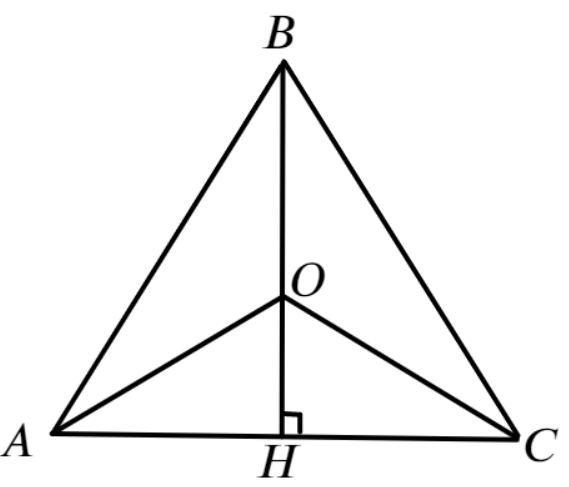
\includegraphics[scale=0.35]{g9-69.png}}
\end{figure}\\
Проведём из вершины высоту $BH$ и отметим на ней центр описанной окружности $O$ (высота является серединным перпендикуляром, поэтому он ей принадлежит). Тогда $HC=AC:2=6,\ OH=\sqrt{10^2-6^2}=8,\ BH=8+10=18,\ S_{\Delta ABC}=\cfrac{1}{2}\cdot18\cdot12=108\text{ см}^2.$\\
